\section{Decentralized Git Workflow}
\label{sec:git}

Git is a distributed version control system that is commonly used in a
centralized workflow. Developers often work using a local Git repository and
coordinate with other developers by pushing their changes to a remote Git
repository that is either hosted by a trusted third party or self-hosted. While
developers are free to host their own remote Git repositories, it is far more
common to rely on a web service such as Github to handle hosting. Github
abstracts away the complexities of repository hosting and also offers developers
additional featues that are not native to Git such as access control, issue
tracking and a pull request system. Developers use a remote protocol such as
HTTP, SSH or Git (packaged with the VCS) to communicate with and transfer data
to the remote repository hosted on Github\cite{gitprotocol}. Ease of use and collaboration features have
solidified Github as a crucial developer productivity tool. However, a
centralized workflow centered around Github also has a number of downsides. If a
user relies on Github, the user also relies on all of Github's dependencies. The
failure of a dependency resulting from a cyberattack can render
Github's services and any hosted code unavailable for a period of
time\cite{dynddos}. Furthermore, any additional repository features such as
payments and governance mechanisms around project direction cannot be directly
integrated into a repository because Github ultimately controls the
remote repository. As long as Github is used as a centralized service to
coordinate and collaborate on a project, these features can only be integrated
into a project if Github chooses to implement them. Consequently, there is
potential value in a decentralized Git workflow that does not rely on a
centralized service like Github to coordinate and collaborate on projects.

\subsection{Mango}

Past work to enable a decentralized Git workflow includes Alex Beregszaszi's Mango, a remote protocol for Git that uses Ethereum smart contracts for remote
repository access control and stores Git objects in decentralized content addressable storage
networks\cite{mango}. The smart contract associated with a repository maintains
a whitelisted set of Ethereum addresses that can push changes to the repository. Although Mango is storage solution agonistic, it is best
served by a decentralized content addressable solution and the initial
implementation uses the Interplanetary File System (IPFS), a peer-to-peer
distributed file system\cite{ipfs}. Git objects are serialized and uploaded to
IPFS which returns the content hash for the objects. Since Git uses the SHA1
hash algorithm, while IPFS is hash algorithm agnostic, a snapshot mapping of Git
SHA1 object hashes to IPFS object hashes is also uploaded to
IPFS\cite{mangoTech}. These IPFS snapshot hashes and Git references are then
stored in an Ethereum smart contract. The smart contract address is used as an
identifier for the repository. Using a command line tool, users can push to and
clone a remote repository using the smart contract address associated with a repository.

\subsection{OpenCollab-CLI and Extensions to Mango}

In order for the Mango protocol to support a decentralized Git workflow that is
comparable in productivity capabilities to a centralized Git workflow using Github, it
needs to offer issue tracking and a pull request system. As a part of our contributions, we
extended the original Mango protocol implementation by modifying the
\textproc{MangoRepo} smart contract to support CRUD operations for issues and
pull requests. We developed the OpenCollab-CLI command line which allows users to manage
issues and pull requests for a repository in a terminal. The command line tool uses Swarm, a distributed storage platform and Ethereum
ecosystem service, rather than IPFS as a decentralized storage
solution\cite{swarm}. However, similar to the original Mango protocol, our
protocol extensions are also storage solution agnostic.

OpenCollab-CLI can be used to push to and clone a remote repository using the
smart contract address associated with a repository as depicted in Figures
\ref{fig:push} and \ref{fig:clone}.

\begin{figure}[]
  \centering
  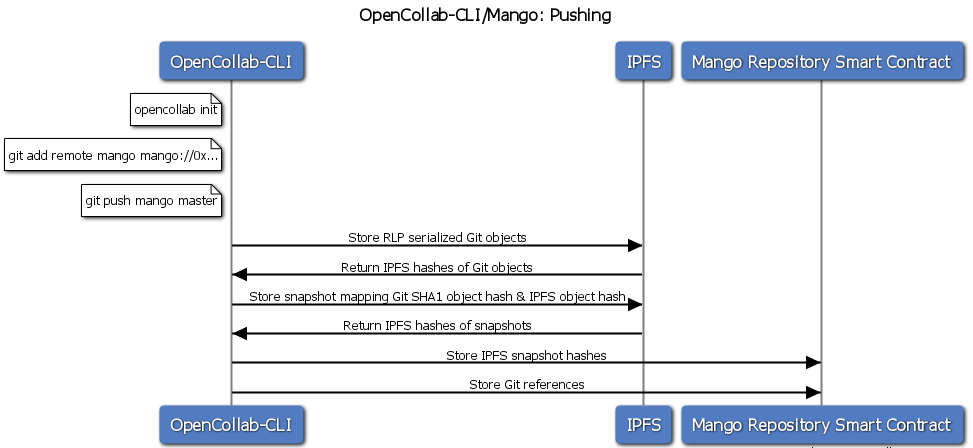
\includegraphics[width=\linewidth,keepaspectratio]{figures/OpenCollab-CLI-Mango-Pushing.png}
  \caption{Pushing to a remote repository using the Mango remote protocol and OpenCollab-CLI}
  \label{fig:push}

\end{figure}

\begin{figure}[]
  \centering
  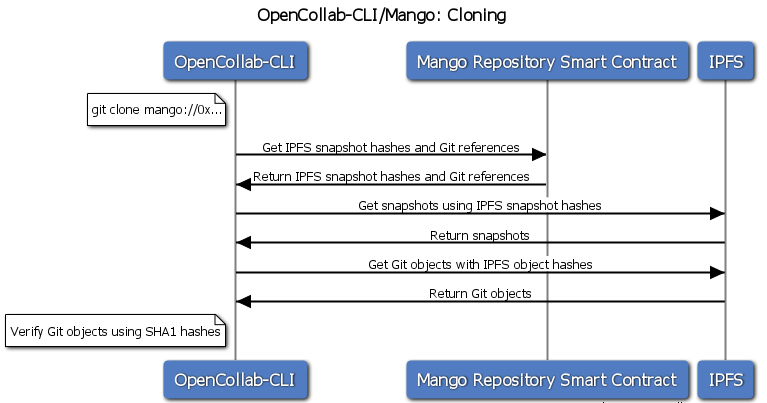
\includegraphics[width=\linewidth,keepaspectratio]{figures/OpenCollab-CLI-Mango-Cloning.png}
  \caption{Cloning a remote repository using the Mango remote protocol and OpenCollab-CLI}
  \label{fig:clone}
\end{figure}

Issue contents are uploaded to Swarm which returns the hash for the contents.
The Swarm hash is then stored in the smart contract for the repository and
mapped to an integer identifier. When using the command line tool, retrieving the contents of an issue consists of
querying the smart contract with the issue identifier and then querying Swarm
using the Swarm hash corresponding to the issue identifier. The process of
creating an issue using OpenCollab-CLI is depicted in Figure \ref{fig:issue}.

\begin{figure}[]
  \centering
  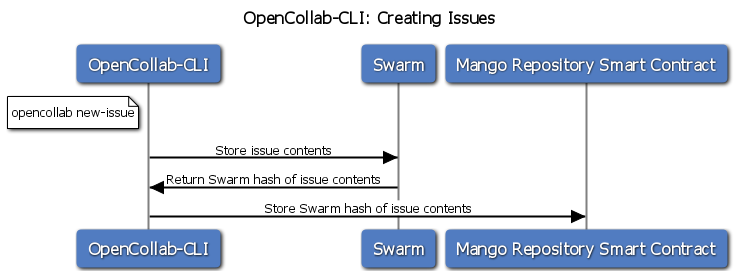
\includegraphics[width=\linewidth,keepaspectratio]{figures/OpenCollab-CLI-Creating-Issues.png}
  \caption{Creating issues using OpenCollab-CLI}
  \label{fig:issue}
\end{figure}

Users can create a pull request with a two step process. First, they need to
fork the project. The command line tool can be used to fork a project locally.
In the project fork, users can initialize a new Mango repository, make relevant
changes and push to the smart contract address associated with the repository fork.
After pushing a project fork, users can use the command line tool to create a
new pull request that references an issue identifier and the contract address
for the repository fork. The process of opening a pull request using
OpenCollab-CLI is depicted in Figure \ref{fig:openPR}.

\begin{figure}[]
  \centering
  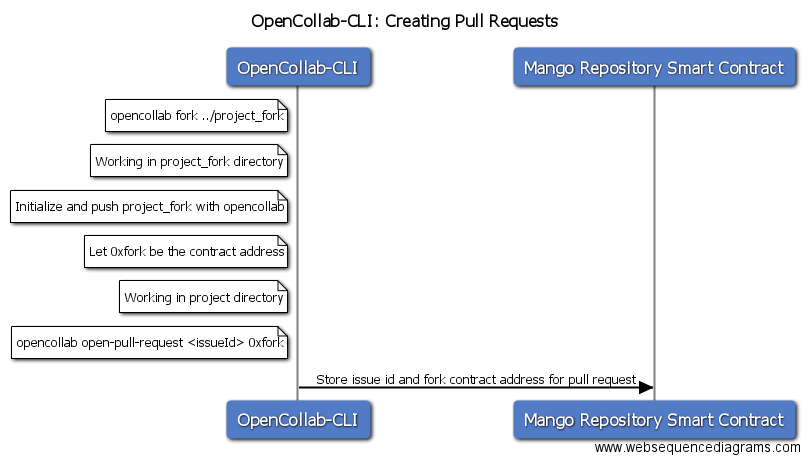
\includegraphics[width=\linewidth,keepaspectratio]{figures/OpenCollab-CLI-Creating-Pull-Requests.png}
  \caption{Creating pull requests using OpenCollab-CLI}
  \label{fig:openPR}
\end{figure}

A project maintainer can merge a pull request with a two step process.
Maintainers can locally clone a repository fork using the contract address
referenced in a pull request. The command line tool can be used to locally merge
a repository fork into the main repository. Then, maintainers can push the
merged changes to the contract address associated with the main repository as
long as their Ethereum address is whitelisted by the repository contract. The
process of merging a pull request using OpenCollab-CLI is depicted in Figure \ref{fig:mergePR}.

\begin{figure}[]
  \centering
  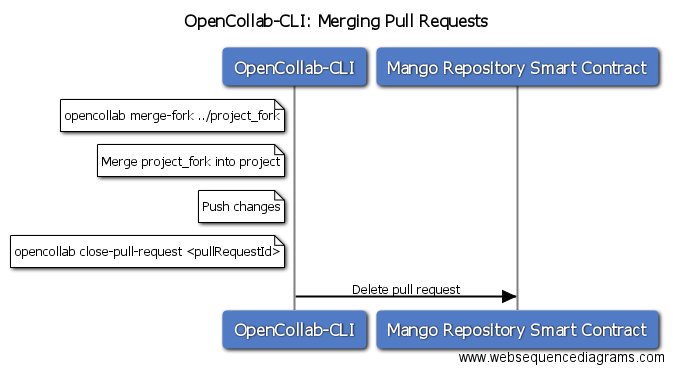
\includegraphics[width=\linewidth,keepaspectratio]{figures/OpenCollab-CLI-Merging-Pull-Requests.png}
  \caption{Merging pull requests using OpenCollab-CLI}
  \label{fig:mergePR}
\end{figure}

OpenCollab-CLI can serve as tool for constructing protocols for open source
software projects that offer additional features such as payments and governance
mechanisms for project direction. The OpenCollab protocol is one such protocol that we describe
in Section \ref{sec:protocol}.

\begin{figure}[]
  \centering
  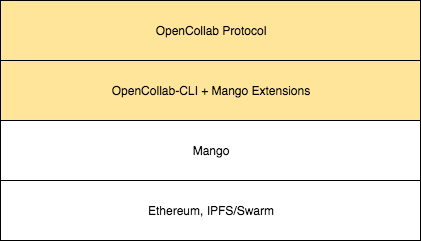
\includegraphics[width=\linewidth,keepaspectratio]{figures/ContributionsStack.png}
  \caption{The technology stack underlying the OpenCollab protocol. The
    layers representing the contributions of this thesis are highlighted}
\end{figure}

\subsection{Future Work}

The OpenCollab-CLI command line tool along with our extensions to the Mango
protocol enable a decentralized Git workflow that not only obviates the need for a
centralized service like Github to coordinate and collaborate for projects, but
also creates the possibility of directly integrating features such as payments and
governance mechanisms directly into a repository at the protocol level. These
contributions serve as neccessary foundation for the OpenCollab blockchain based
protocol which is described in the next section. At the moment, the
OpenCollab-CLI command line tool and the OpenCollab protocol are separate.
Future work would include upgrading OpenCollab-CLI to be
compatible with the OpenCollab protocol.

% Local Variables:
% org-ref-default-bibliography: ../bib/git.bib
% End:
